\NewScheme{\SPOR}{SPOR}

\subsection{Message Passing: Stateless Predictive Onion Routing \(\SPOR\)}
\label{sec:message_passing}

\NewAlgorithm{\Send}{Send}
\NewAlgorithm{\Fwd}{Forward}
\NewAlgorithm{\Recv}{Receive}
\NewVariable{\rdv}{rdv}

We have the Stateless Predictive Onion Routing scheme, \SPOR, which provides 
probabilistically onion-routed message passing.
Instead of providing only one address per hop in the route (as in \eg 
Tor~\cite{Tor}), \(\SPOR\) provides several alternatives for the next hop 
depending on their probability of being online.
To do this, \(\SPOR\) provides stateless algorithms for the onion-routing.

\(\SPOR\) provides three algorithms: \(\SPOR[\Send]\) (\cref{SPORSend}), 
\(\SPOR[\Fwd]\) (\cref{SPORFwd}) and \(\SPOR[\Recv]\) (\cref{SPORRecv}).
Say Alice wants to send a message \(m\) to Bob.
Bob uses \(\SPOR[\Recv]\) to create a probabilistic onion route \(H_\rdv\) from 
a rendez-vous point to his own device swarm --- all the hops on the route are 
chosen by Bob uniformly at random.
Bob gives \(H_\rdv\) to Alice using an out-of-band channel, \eg using his phone.
Alice uses \(\SPOR[\Send]\) at some later time to send the message to Bob using 
any of her devices.
\(\SPOR[\Send]\) extends the route \(H_\rdv\) with some hops of Alice's choosing 
(uniformly randomly chosen), then starts to forward the message (using 
\(\SPOR[\Fwd]\)) through the hops on the route to Bob.
This process is illustrated in \cref{fig:file-exchange}.

\begin{figure}
  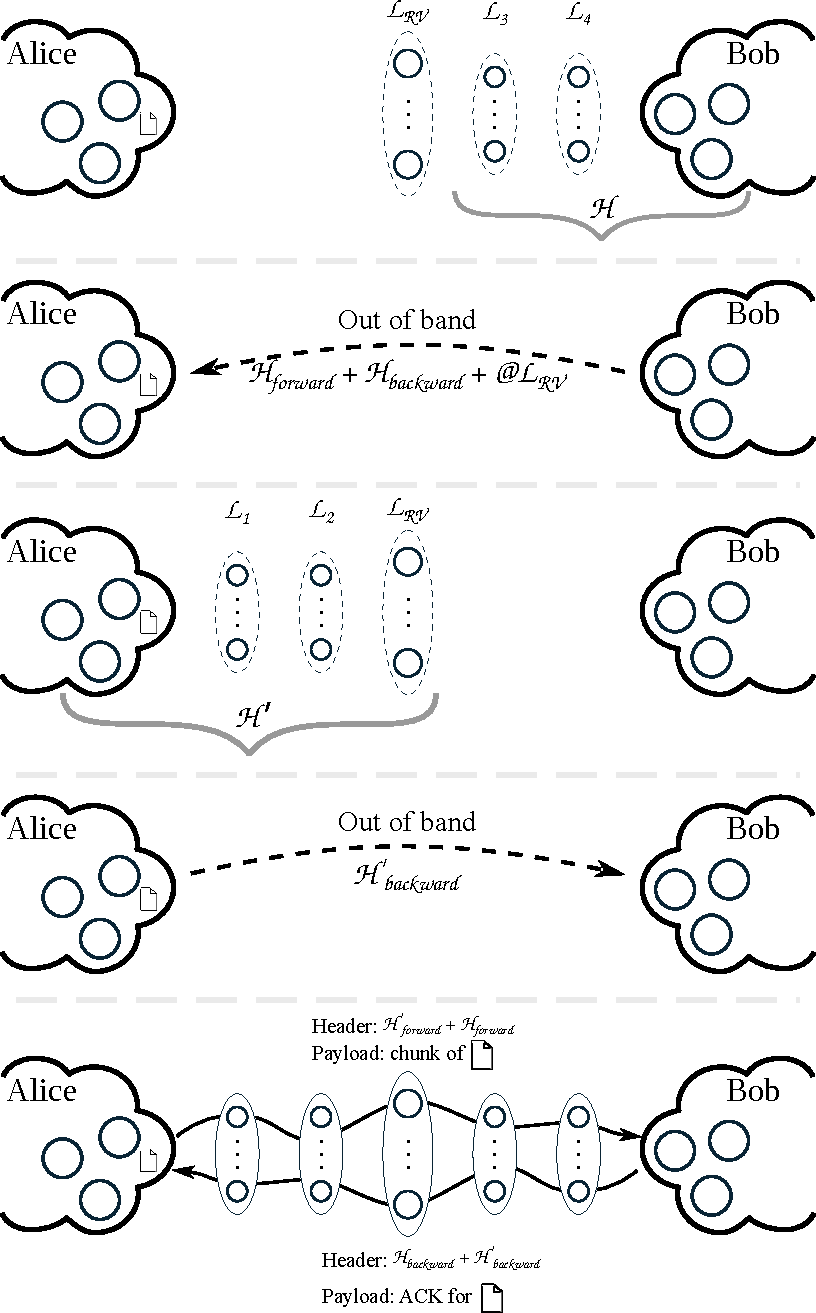
\includegraphics[width=\linewidth]{figures/file_exchange.pdf}
  \caption{\label{fig:file-exchange}%
    A schematic of Alice and Bob sending a message using \(\SPOR\).
  }
\end{figure}

\NewAlgorithm{\ExtendRoute}{ExtendRoute}
\NewAlgorithm{\CreateOnionLayer}{CreateOnionLayer}

\begin{figure}
  \begin{algorithmic}
    \Require{%
      $H$ is a header of the form \(D\concat H'\) or \(D\concat \top\), where 
      \(D\) is a set of device addresses.
      $\pk_D$ is the public key of device set $D$.
      $L$ is the length of the route,
      $\theta$ is the threshold of probability of failure.%
    }
    \Function{\ExtendRoute}{$H, L, \theta$}
      \If{$L\leq 0$}
        \State \Return $H$
      \EndIf
      \State $D\gets \CreateOnionLayer[\theta]$
      \State $H\gets D\concat \DeBEenc[\mpk, D, H]$
      \State \Return $\ExtendRoute[H, L-1, \theta]$
    \EndFunction

    \Function{\CreateOnionLayer}{$\theta$}
      \State $(d, \pk_d, p_d)\gets \GetRandomPeer$
      \Comment We use \(d\) as shorthand for this tuple.
      \State $D\gets \{d\}$
      \While{$\prod_{d\in D} p_d > \theta$}
        \State $d\gets \GetRandomPeer$
        \State $D\gets D\cup \{d\}$
      \EndWhile
      \State \Return $D$
    \EndFunction
  \end{algorithmic}
  \caption{\label{ExtendRoute}%
    The \(\ExtendRoute\) algorithm extends a route \(H\) with \(L\) hops and 
    failure threshold of \(\theta\) for each hop in the route.
    Thus the probability of failure for the extension is \(1 - (1 - \theta)^L\).
    The function \(\GetRandomPeer\) is any random peer-sampling algorithm.
  }
\end{figure}

\NewAlgorithm{\Store}{Store}
\NewAlgorithm{\Dec}{Dec}
\NewVariable{\sk}{sk}

\begin{figure}
  \begin{algorithmic}
    \Require{%
      $D$ is the set of alternative recipient devices.
    }
    \Function{\SPOR[\Recv]}{$D$}
      \State $H_\rdv\gets \ExtendRoute[D\concat \top, L, \theta]$
      \State \Return $H_\rdv$
        \Comment{Give to sender out-of-bound.}
    \EndFunction

    \Function{\Store}{$m$}
      \State $m\gets \DeBEdec[\mpk, \sk, c_m]$
      \If{$m = \bot$}
        \State \Return $\bot$
      \EndIf
      \State Store $m$ to disk.
      \State \Return $\top$
    \EndFunction
  \end{algorithmic}
  \caption{\label{SPORRecv}%
    The \(\SPOR[\Recv]\) algorithm prepares the recipient for receiving a file.
    It creates a probabilistic onion-route from a rendez-vous point to its own 
    devices and returns the route to the sender.
    The \(\Store\) algorithm is used by the local \(\SPOR[\Fwd]\) algorithm to 
    store messages intended for itself.
  }
\end{figure}

\begin{figure}
  \begin{algorithmic}
    \Require{%
      $m$ is the message to be sent,
      $H_\rdv$ is the onion-route given by the recipient.
    }
    \Function{\SPOR[\Send]}{$H_\rdv, m$}
      \State $H\gets \ExtendRoute[H_\rdv, L, \theta]$
      \State $D\concat C_H\gets H_\rdv$
      \For{$d\in D$}
        \Comment{Uniformly randomly chosen}
        \If{$d\method \Fwd[C_H, m] \neq \bot$}
          \State \Return $\top$
        \EndIf
      \EndFor
      \State \Return $\bot$
    \EndFunction
  \end{algorithmic}
  \caption{\label{SPORSend}%
    The \(\SPOR[\Send]\) algorithm extends the route \(H_\rdv\) (using 
    \(\ExtendRoute\), \cref{ExtendRoute}) and sends the message \(m\) down the 
    extended route using the \(\SPOR[\Fwd]\) algorithm (\cref{SPORFwd}).
    The first node of \(H_\rdv\) is the rendez-vous point selected by the 
    recipient.
  }
\end{figure}

\begin{figure}
  \begin{algorithmic}
    \Require{$\pk, \sk$ is the public--private key-pair of the node.}
    \Function{\SPOR[\Fwd]}{$C_H, m$}
      \State $H\gets \DeBEdec[\mpk, \sk, C_H]$
      \If{$H = \bot$}
        \State \Return $\bot$
      \EndIf
      \State $\{d_i\}\concat C_H'\gets H$
      \If{$C_H' = \top$}
        \State \Return $\Store[m]$
      \EndIf
      \For{$d\in \{d_i\}$}
        \Comment{Uniformly randomly chosen}
        \If{$d\method \Fwd[C_H', m] \neq \bot$}
          \State \Return $\top$
        \EndIf
      \EndFor
      \State \Return $\bot$
    \EndFunction
  \end{algorithmic}
  \caption{\label{SPORFwd}%
    The \(\SPOR[\Fwd]\) algorithm forwards \(m\) down the route \(H\), obtained 
    by decrypting \(C_H\) with the node's associated private key.
    The special value \(H = \top\) indicated the end of the route, thus \(c_m\) 
    is intended for the local node and \(c_m\) is instead sent to disk using 
    \(\Store\) (\cref{SPORRecv}).%
  }
\end{figure}

